% How trace_fn() turns an R function into an AnvlGraph: the function and the call; the R
% variables of the function while it is traced; the graph it records, with its inputs and output
% in the accent color; and numbered notes on what happens. The branch that is never evaluated is
% gray. The graph is printed by anvl 0.6.0. Shared style in style.tex.
% Build: make figures/tracing.pdf
\documentclass[tikz, border = 6pt]{standalone}
% The style shared by the TikZ figures of the paper (overview.tex, tracing.tex, async.tex):
% fonts, the colors of the packages, the highlight color, and the styles of boxes, headings,
% numbered badges, and notes. benchmarks/plots.R uses the same colors and font for the plots.
\usepackage[T1]{fontenc}
\usepackage{lmodern}
\usetikzlibrary{positioning, calc, fit, backgrounds, matrix, arrows.meta}

% Colors of the packages, as in the overview figure (after the mlr3torch figures).
\definecolor{tealframe}{HTML}{21908c}
\definecolor{lightbox}{HTML}{e4f1f1}
\definecolor{viridis1}{HTML}{8e6698}
\definecolor{viridis8}{HTML}{ccea84}
\definecolor{modelgrey}{HTML}{e5e5e5}
\colorlet{cr}{white}
\colorlet{canvl}{lightbox}
\colorlet{cstablehlo}{viridis1!22}
\colorlet{cpjrt}{viridis8!45}
\colorlet{cquickr}{modelgrey}

% The highlight color: the part of a figure that shows its point.
\colorlet{accent}{tealframe}

\newcommand{\cd}[1]{\texttt{#1}}
\newcommand{\hl}[1]{\textcolor{accent}{#1}}

\tikzset{
  % a box around a part of a figure, and its heading
  box/.style = {rounded corners = 2pt, inner sep = 5pt},
  plainbox/.style = {box, draw = black!25, fill = black!4},
  framebox/.style = {box, draw = black!40},
  accentbox/.style = {box, draw = accent!80!black, fill = accent!7},
  head/.style = {font = \footnotesize\bfseries, text = black!70, anchor = south west,
    inner sep = 1pt},
  % a number that links a part of a figure to a note
  badge/.style = {circle, fill = black!65, text = white, font = \sffamily\tiny\bfseries,
    inner sep = 0pt, minimum size = 3.2mm, anchor = base},
  note/.style = {font = \footnotesize, align = left, text width = 7.4cm, anchor = north west,
    inner sep = 0pt, execute at begin node = {\thickmuskip = 5mu}},
  % lines of code or of a printed graph, followed by columns of badges
  lines/.style = {matrix of nodes, row sep = {3.9mm, between origins}, column sep = 2pt,
    nodes = {anchor = base west, inner sep = 0.5pt, font = \ttfamily\scriptsize}},
  % rows of a name and its value(s)
  fields/.style = {matrix of nodes, row sep = {3.9mm, between origins}, column sep = 2pt,
    nodes = {anchor = base west, inner sep = 0.5pt, font = \ttfamily\scriptsize},
    column 1/.style = {nodes = {text = black!55}}},
  flow/.style = {-{Stealth[length = 1.6mm]}, black!55, thin}
}

% A note: its text at #2, numbered #1 in a badge hanging to its left.
\newcommand{\note}[3]{
  \node[note] (#1) at #2 {#3};
  \node[badge, font = \sffamily\scriptsize\bfseries, minimum size = 3.8mm, anchor = north east]
    at ($(#1.north west) + (-0.15, 0.04)$) {#1};
}


% Inputs and output of the graph.
\newcommand{\io}[1]{\hl{#1}}
% Code that is never evaluated.
\newcommand{\unused}[1]{\textcolor{black!40}{#1}}

\tikzset{note/.append style = {text width = 7.0cm}, code/.style = {lines, column sep = 5pt, column 2/.style = {nodes = {badge}}, column 3/.style = {nodes = {badge}}}}

\begin{document}
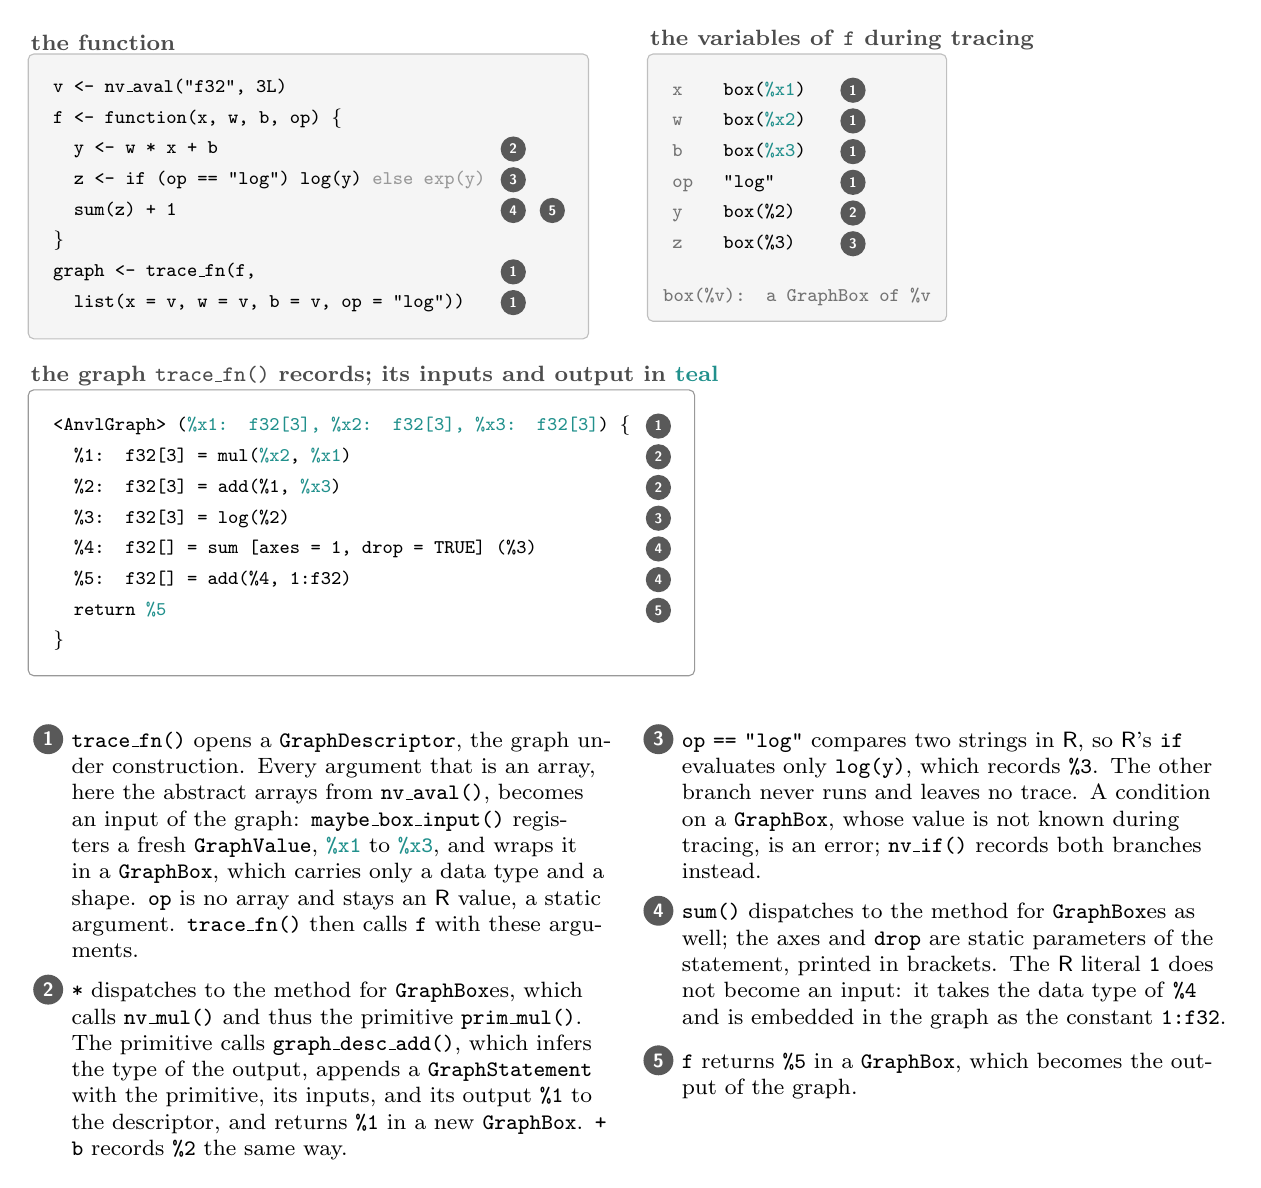
\begin{tikzpicture}

  \matrix[code] (code) at (0, 0) {
    v <- nv\_aval("f32", 3L) & \\
    f <- function(x, w, b, op) \{ & \\
    \ \ y <- w * x + b & 2 \\
    \ \ z <- if (op == "log") log(y) \unused{else exp(y)} & 3 \\
    \ \ sum(z) + 1 & 4 & 5 \\
    \} & \\
    graph <- trace\_fn(f, & 1 \\
    \ \ list(x = v, w = v, b = v, op = "log")) & 1 \\
  };
  \begin{scope}[on background layer]
    \node[plainbox, fit = (code)] (codebox) {};
  \end{scope}
  \node[head] at (codebox.north west) {the function};

  % Right of the function: its variables while it is traced.
  \matrix[fields, anchor = north west] (vars) at ($(code.north east) + (1.1, 0)$) {
    x &[8pt] box(\io{\%x1}) &[10pt] |[badge]| 1 \\
    w & box(\io{\%x2}) & |[badge]| 1 \\
    b & box(\io{\%x3}) & |[badge]| 1 \\
    op & "log" & |[badge]| 1 \\
    y & box(\%2) & |[badge]| 2 \\
    z & box(\%3) & |[badge]| 3 \\
  };
  \node[font = \ttfamily\scriptsize, text = black!55, anchor = north west, inner sep = 0.5pt]
    (boxlegend) at ($(vars.south west) + (0, -0.25)$) {box(\%v): a GraphBox of \%v};
  \begin{scope}[on background layer]
    \node[plainbox, fit = (vars) (boxlegend)] (varsbox) {};
  \end{scope}
  \node[head] at (varsbox.north west) {the variables of \cd{f} during tracing};

  \matrix[code, below = 1.0 of code.south west, anchor = north west] (graph) {
    <AnvlGraph> (\io{\%x1: f32[3], \%x2: f32[3], \%x3: f32[3]}) \{ & 1 \\
    \ \ \%1: f32[3] = mul(\io{\%x2}, \io{\%x1}) & 2 \\
    \ \ \%2: f32[3] = add(\%1, \io{\%x3}) & 2 \\
    \ \ \%3: f32[3] = log(\%2) & 3 \\
    \ \ \%4: f32[] = sum [axes = 1, drop = TRUE] (\%3) & 4 \\
    \ \ \%5: f32[] = add(\%4, 1:f32) & 4 \\
    \ \ return \io{\%5} & 5 \\
    \} & \\
  };
  \begin{scope}[on background layer]
    \node[framebox, fit = (graph)] (graphbox) {};
  \end{scope}
  \node[head] at (graphbox.north west)
    {the graph \cd{trace\_fn()} records; its inputs and output in \io{teal}};

  % The notes go below the boxes, in two columns: 1 and 2 on the left, 3 to 5 on the right.
  \coordinate (notes) at ($(graphbox.south west) + (0.55, -0.7)$);
  \coordinate (notes2) at ($(notes) + (7.75, 0)$);
  \note{1}{(notes)}
    {\cd{trace\_fn()} opens a \cd{GraphDescriptor}, the graph under construction. Every
     argument that is an array, here the abstract arrays from \cd{nv\_aval()}, becomes an
     input of the graph: \cd{maybe\_box\_input()} registers a fresh \cd{GraphValue},
     \io{\cd{\%x1}} to \io{\cd{\%x3}}, and wraps it in a \cd{GraphBox}, which carries only a
     data type and a shape. \cd{op} is no array and stays an \textsf{R} value, a static
     argument. \cd{trace\_fn()} then calls \cd{f} with these arguments.}
  \note{2}{($(1.south west) + (0, -0.3)$)}
    {\cd{*} dispatches to the method for \cd{GraphBox}es, which calls \cd{nv\_mul()} and
     thus the primitive \cd{prim\_mul()}. The primitive calls \cd{graph\_desc\_add()}, which
     infers the type of the output, appends a \cd{GraphStatement} with the primitive, its
     inputs, and its output \cd{\%1} to the descriptor, and returns \cd{\%1} in a new
     \cd{GraphBox}. \cd{+ b} records \cd{\%2} the same way.}
  \note{3}{(notes2)}
    {\cd{op == "log"} compares two strings in \textsf{R}, so \textsf{R}'s \cd{if} evaluates
     only \cd{log(y)}, which records \cd{\%3}. The other branch never runs and leaves no
     trace. A condition on a \cd{GraphBox}, whose value is not known during tracing, is an
     error; \cd{nv\_if()} records both branches instead.}
  \note{4}{($(3.south west) + (0, -0.3)$)}
    {\cd{sum()} dispatches to the method for \cd{GraphBox}es as well; the axes and
     \cd{drop} are static parameters of the statement, printed in brackets. The \textsf{R}
     literal \cd{1} does not become an input: it takes the data type of \cd{\%4} and is
     embedded in the graph as the constant \cd{1:f32}.}
  \note{5}{($(4.south west) + (0, -0.3)$)}
    {\cd{f} returns \cd{\%5} in a \cd{GraphBox}, which becomes the output of the graph.}

\end{tikzpicture}
\end{document}
